\numberedchapter{Preliminary Work}

\numberedsection{Datasets Description}

\newcommand{\cifar}{\href{https://www.cs.toronto.edu/~kriz/cifar.html}{\texttt{cs.toronto.edu/\string~kriz/cifar.html}}}
\newcommand{\scaledcifar}{\href{https://www.kaggle.com/datasets/joaopauloschuler/cifar10-64x64-resized-via-cai-super-resolution}{\texttt{kaggle.com/datasets/joaopauloschuler/cifar10-64x64-resized-via-cai-super-resolution}}}
\newcommand{\coco}{\href{https://cocodataset.org/}{\texttt{cocodataset.org}}}

In this segment of the discussion, an in-depth exploration of the two datasets, integral to the development of the project, will be undertaken. The forthcoming discourse will clarify the specifics, characteristics and distinctive aspects of each dataset, delivering a comprehensive understanding of their role within the scope of the project.

\numberedsubsection{CIFAR-10}

The \textbf{CIFAR-10}\footnote{\cifar} (Canadian Institute for Advanced Research) dataset is a widely used dataset for machine learning and computer vision research. It contains a total of 60,000 images divided into 10 distinct classes: aeroplanes, cars, birds, cats, deer, dogs, frogs, horses, ships and trucks, as depicted in \autoref{fig:cifar}. Each class contains 6,000 images and the dataset is further divided into \textbf{50,000 training images} and \textbf{10,000 testing images}. The images in the CIFAR-10 dataset are colour and relatively small, each with a dimension of $\symbf{32\stimes32}$ pixels~\supercite{cifar}. The dataset, a ubiquitous tool for machine learning and computer vision initiatives, presents unique characteristics that can be both advantageous and disadvantageous in the context of inpainting degraded colour images:
\begin{itemize}[leftmargin=1.5em]
    \setlength\itemsep{0.2cm}

    \item \textbf{Variety of classes} -- The CIFAR-10 dataset's broad variety of categories provides a balanced and diverse training platform, enabling a model to learn intricate features and distinctions across different classes.

    \item \textbf{Established benchmark} -- Owing to its extensive use in academic research, it serves as an excellent benchmark for evaluating the effectiveness of different algorithms. Numerous state-of-the-art models have been tested on this dataset and their performances have been recorded, facilitating a comparative study.

    \item \textbf{Size and complexity} -- Despite the relatively small size of the images, they are complex enough to pose a substantial challenge, thus testing the robustness of machine learning models.

    \item \textbf{Low resolution} -- The primary limitation of the CIFAR-10 dataset is the low resolution of the images. While this reduces computational requirements, it could potentially hamper the ability to inpaint high-resolution images as the model may not learn sufficient high-frequency details.

    \item \textbf{Limited domain} -- Despite the variety of classes, the CIFAR-10 dataset is relatively limited in its representation of the real world. The classes are constrained and there's an absence of images depicting complex scenes, variations in lighting or images captured from varying perspectives. Hence, a model might not perform well on more diverse and complex images.
\end{itemize}

\begin{figure}[ht]
    \centering
    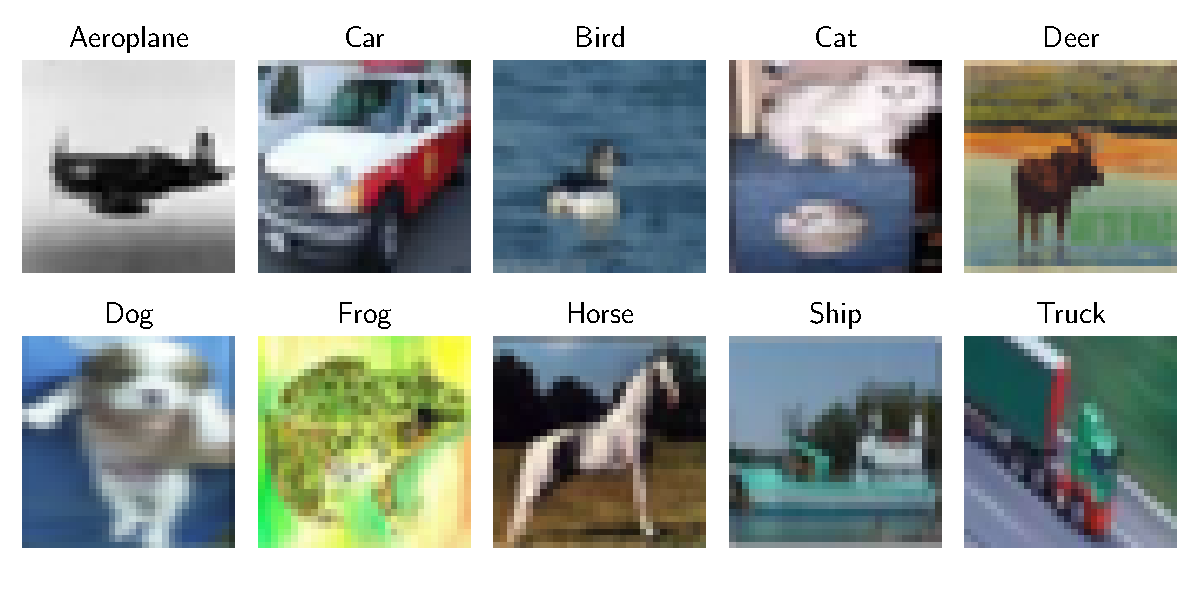
\includegraphics[width=\textwidth]{preliminary-work/cifar10.pdf}
    \caption{Image samples from the CIFAR-10 dataset}
    \label{fig:cifar}
\end{figure}

In the search for addressing the challenge of image inpainting, a notable constraint is encountered when leveraging the standard CIFAR-10 dataset: the diminutive image size of $32\stimes32$ pixels. The network architectures that are going to be presented in the \hyperref[section:solutions]{subsequent chapter} involve deep convolutional networks, which are characterized by a progressive reduction of spatial dimensions as we move deeper into the network. This inherent feature of such architectures is incompatible with the small size of standard CIFAR-10 images, leading to difficulties in the meaningful extraction of higher-level features due to rapid downscaling. To circumvent this limitation and ensure a sustainable depth of learning, we opt for an upscaled version of the CIFAR-10 dataset, presenting images at a resolution of $\symbf{64\stimes64}$ pixels\footnote{\scaledcifar}, as illustrated in \autoref{fig:cifar-upscaled}. This approach retains the diverse content of the original dataset while accommodating the requirements of our selected deep-learning models. Consequently, the larger images facilitate the capture of more detailed features and enable a more robust learning process, improving the potential performance of the inpainting task at hand.

\begin{figure}[ht]
    \centering
    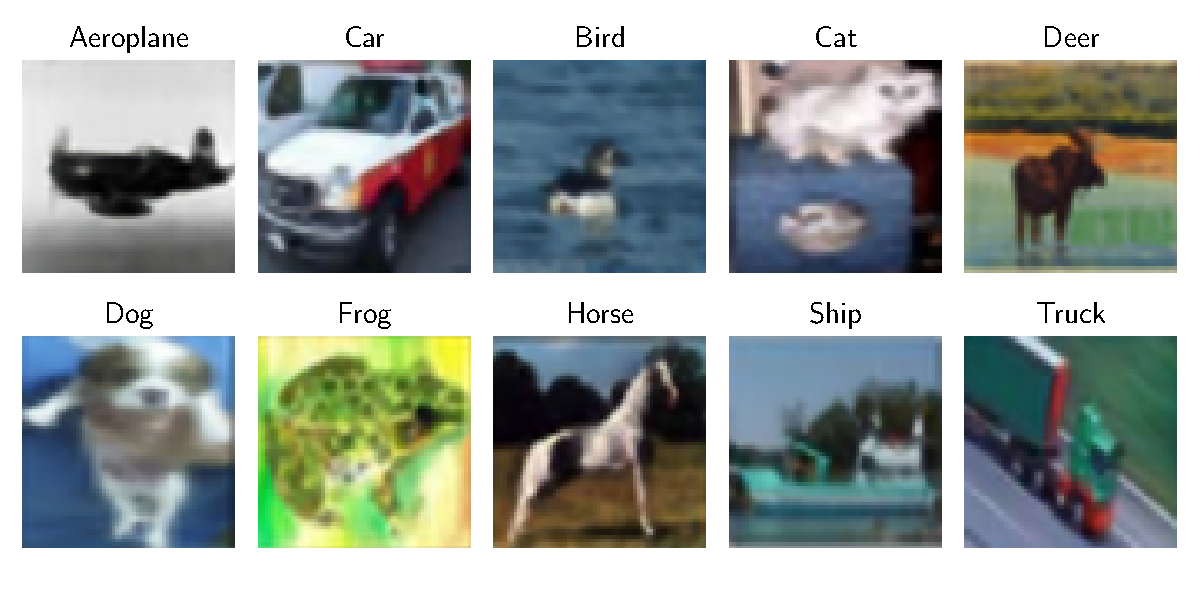
\includegraphics[width=\textwidth]{preliminary-work/cifar10-upscaled.pdf}
    \caption{Upscaled of the same image samples from the CIFAR-10 dataset}
    \label{fig:cifar-upscaled}
\end{figure}

The selection and usage of the CIFAR-10 dataset and its upscaled version in the incipient phases of this project proved to be an instrumental decision. With a principal goal of developing and refining the image inpainting architectures, the CIFAR-10 dataset offered a convenient yet diverse array of images for initial testing and training. The modest size of the dataset, coupled with the relatively higher resolution of the upscaled version, facilitated an environment favourable to rapid experimentation and iterative improvement of the models. This combination enabled the project to strike a crucial balance: extracting meaningful, high-level features critical for the inpainting task while ensuring that model training and testing could be executed within reasonable time frames, a process that would have been substantially more challenging with larger and more complex datasets.

\numberedsubsection{Common Objects in Context}

The \textbf{Common Objects in Context}\footnote{\coco} (COCO) database is a large-scale, richly annotated dataset designed to spur advancements in object detection, segmentation, person keypoints detection, stuff segmentation and caption generation. The dataset comprises 330,000 colour images of varying dimensions, encompassing 1.5 million object instances across 90 categories~\supercite{coco}, as represented in \autoref{fig:coco}. In the context of degraded colour image inpainting, the COCO dataset brings its own strengths and potential weaknesses:
\begin{itemize}[leftmargin=1.5em]
    \setlength\itemsep{0.2cm}

    \item \textbf{High diversity and complexity of scenes} -- COCO contains images with complex everyday scenes, often with multiple objects per image, providing a diverse and challenging learning environment. But this complexity is beneficial for developing a more robust inpainting model that can handle real-world scenarios.

    \item \textbf{Large scale} -- The sheer number of images and object instances is an advantage for training deep learning models, which often benefit from larger datasets.

    \item \textbf{High resolution} -- Images in the COCO dataset are of higher resolution compared to CIFAR-10. This provides more detailed visual information, which is crucial for a task such as image inpainting.

    \item \textbf{Processing power and preparation time} -- The size and complexity of the COCO dataset require more computational resources to process, which slows down model training. Also, given the dataset's richness and diversity, preprocessing and setting up the data for this task is more time-consuming compared to the simpler CIFAR-10 dataset.
\end{itemize}

\begin{figure}[ht]
    \centering
    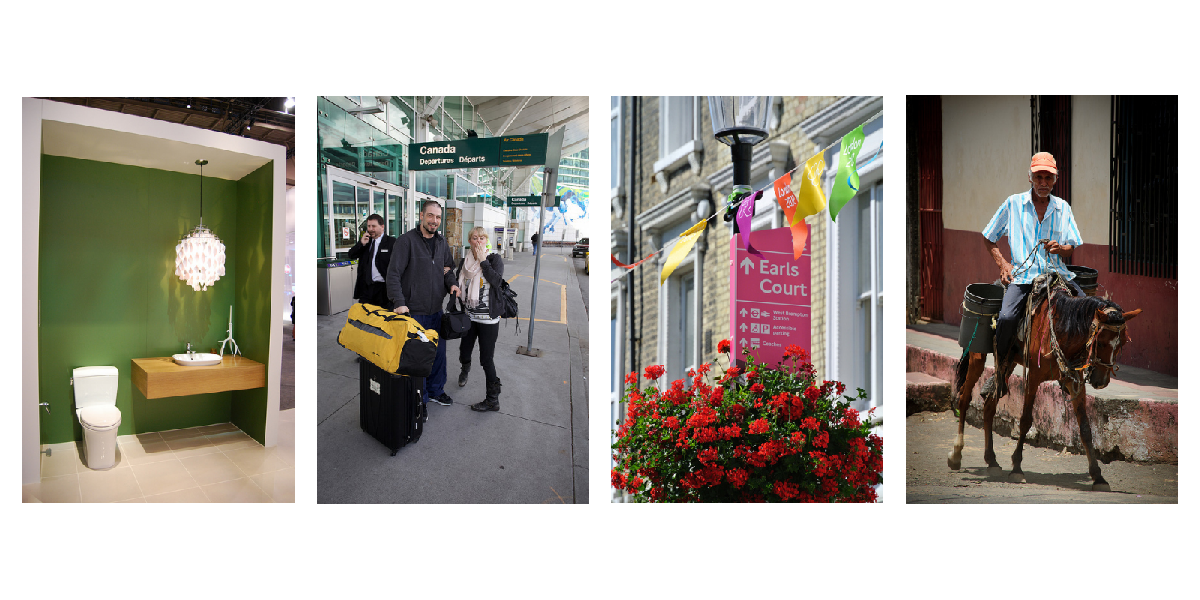
\includegraphics[width=\textwidth]{preliminary-work/coco.pdf}
    \caption{Image samples from the COCO dataset}
    \label{fig:coco}
\end{figure}

Following the initial development and refinement of the models using the CIFAR-10 dataset, the transition was made to the Common Objects in Context dataset for the crucial phases of final model training, testing and evaluation. The choice of the dataset served as a strategic operation designed to elevate the inpainting system's performance in real-world scenarios. COCO's complex, high-resolution images and various object instances provided a rich learning environment that far exceeded the simplified scenarios presented by CIFAR-10. While more computationally demanding, the extensive array of real-world scenes in the dataset ultimately afforded a broader and deeper understanding of varied contexts and challenges in image inpainting.

To conclude, the datasets used in this project were the upscaled version of CIFAR-10 and COCO. The CIFAR-10 was used in its original form, maintaining the initial division of training and testing sets. In contrast, the COCO dataset was further partitioned, being divided into a \textbf{training set of 80,000 images}, a \textbf{testing set of 20,032 images} and a \textbf{validation set of 20,032 images}, while the rest up to 330,000 were discarded due to hardware constraints. The specific number of 20,032 for the test and validation sets was intentionally chosen to be compatible with the batch size employed in the model training process.

\numberedsection{Image Pre-processing}\label{section:preprocess}

\textbf{Data pre-processing} is an indispensable step in the machine learning pipeline. This stage aims to convert raw, unprocessed data into a structured format that is suitable for machine learning algorithms. As revealed in \autoref{fig:process}, the steps constitute loading the image dataset, performing random cropping, generating degraded images through the application of masks, normalizing the images and caching the processed dataset.
\begin{figure}[ht]
    \centering
    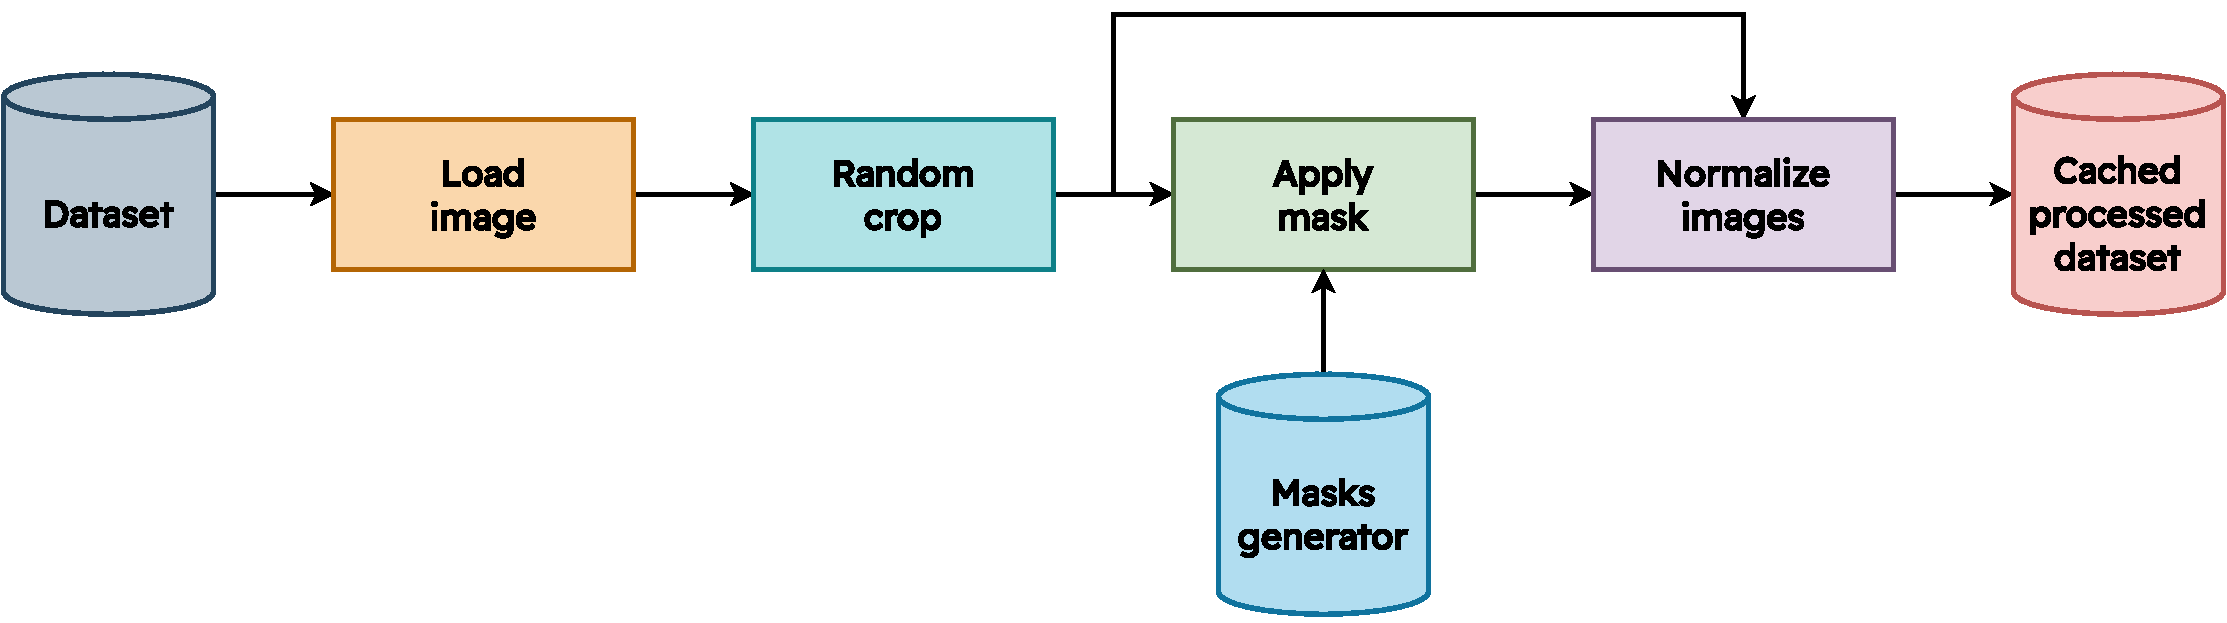
\includegraphics[width=\textwidth]{preliminary-work/pipeline.pdf}
    \caption{Image pre-processing pipeline with masks generator}
    \label{fig:process}
\end{figure}

\unnumberedsubsection{Loading of the image dataset}

The initial step in the pre-processing pipeline involves preparing and loading the image dataset. This process begins with sourcing the images from the internet. Once downloaded, these images are partitioned into distinct subsets for training, testing and validation purposes. This division is performed only once to ensure consistency across experimental iterations. Thereafter, these datasets are imported into the system by reading them from the disk and loading them into the Random Access Memory (RAM). This loading step is crucial as it enables efficient and speedy access to the images during the next processing operations.

\unnumberedsubsection{Random cropping of images}

Upon the successful loading of the images, the next step is the application of random cropping, a process specifically used when handling the COCO dataset. This decision is driven by two primary factors. Firstly, due to hardware limitations, the full processing of high-resolution images, which can contain millions of pixels, becomes computationally demanding. By focusing on a random subset of these pixels, the dimensionality of the dataset is effectively reduced, thereby significantly enhancing computational efficiency. Secondly, the application of random cropping is instrumental in obtaining images of uniform size (chosen $\symbf{128\stimes128}$), a prerequisite for the employed network architectures.
\begin{figure}[h!]
    \centering
    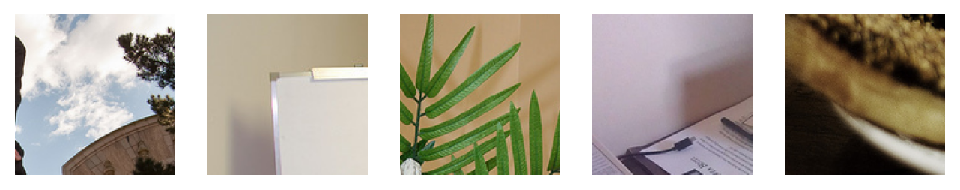
\includegraphics[width=\linewidth]{preliminary-work/images.pdf}
    \caption{Random cropped regions from images}
    \label{fig:random-crop}
\end{figure}

Moreover, as highlighted in \autoref{fig:random-crop}, random cropping serves as a form of \textbf{data augmentation}. This technique, by increasing the diversity of the training data, aids in mitigating the risk of overfitting, thereby enhancing the generalization capability of the model. Thus, the process of random cropping, while primarily employed due to hardware constraints and the necessity of uniform image sizes, also contributes significantly to the robustness of the model.

\unnumberedsubsection{Application of masks}\label{section:mask}

The subsequent step in the pipeline involves the generation and application of masks. Within the scope of image processing, a mask is a binary image that delineates which pixels of an image should be subjected to processing. For this particular task, masks are employed to demarcate the degraded regions within the cropped areas of the images that necessitate inpainting.
\begin{figure}[ht]
    \centering
    \captionsetup[subfigure]{justification=centering}
    \begin{subfigure}[ht]{\linewidth}
        \centering
        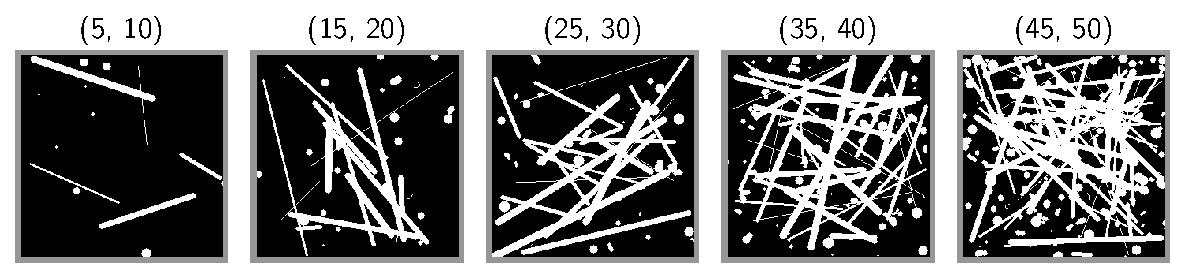
\includegraphics[width=\textwidth]{preliminary-work/random_shapes.pdf}
        \caption{Masks generated using random shapes (lines, circles and distorted ellipses)}
        \label{fig:random_shapes}
    \end{subfigure}
    \vskip\baselineskip
    \begin{subfigure}[ht]{\linewidth}
        \centering
        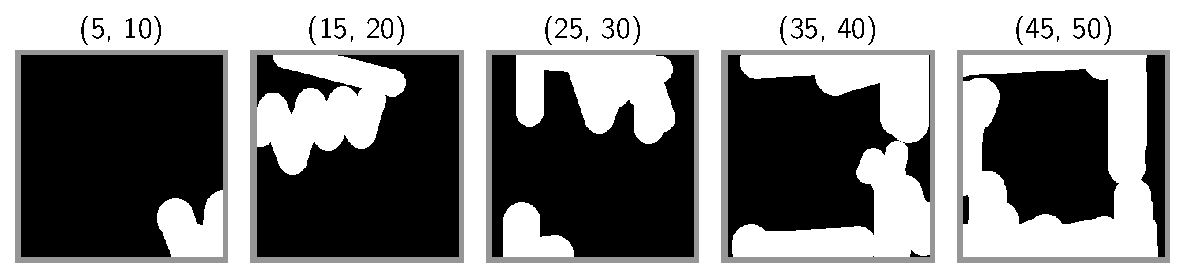
\includegraphics[width=\textwidth]{preliminary-work/freeform.pdf}
        \caption{Mask generated using the modified freeform algorithm (brush-like strokes)}
        \label{fig:freeform}
    \end{subfigure}
    \caption{Comparison of generated masks}
    \label{fig:mask-comp}
\end{figure}

As illustrated in \autoref{fig:random_shapes}, the generation of these masks was initially accomplished using a simple algorithm that produced random shapes, such as lines, circles and distorted ellipses. This approach provided a basic method for creating diverse and randomly degraded regions within the images. However, to enhance the realism and complexity of the degradation, the mask generation process was later updated to incorporate an algorithm derived from \cite{free-form-inpainting}. This updated algorithm generates brush-like strokes, as presented in \autoref{fig:freeform}, thereby creating masks that simulate more natural and realistic degradation patterns.

A key aspect of the mask generation process is the adherence to what is termed a \textbf{degradation ratio interval} (DRI), as seen in the titles of the two previously mentioned figures. This is a predefined interval that specifies, in percentages, the area of the image that should be covered by the degradation. The degradation ratio interval thus provides a control mechanism for the extent of degradation introduced into the images, ensuring a balanced and controlled distribution of degradation across the dataset.

Regardless of whether they are produced by the initial or the updated algorithm, these masks serve a pivotal role in the pre-processing pipeline. They are applied to the cropped regions of the images, with the '1' values in the mask signifying the pixels in the image that should be regarded as degraded, as illustrated in \autoref{fig:masked-comp}. This process of applying the masks effectively transforms the original images into degraded versions, where degraded regions have the maximum attainable pixel value (255 for an 8-bit image).

\emph{Note}: The masks and masked images depicted in the preceding figures are framed with a slight grey border, a design choice implemented to enhance their distinguishability and facilitate easier visual interpretation for the reader.
\begin{figure}[ht]
    \centering
    \captionsetup[subfigure]{justification=centering}
    \begin{subfigure}[ht]{\linewidth}
        \centering
        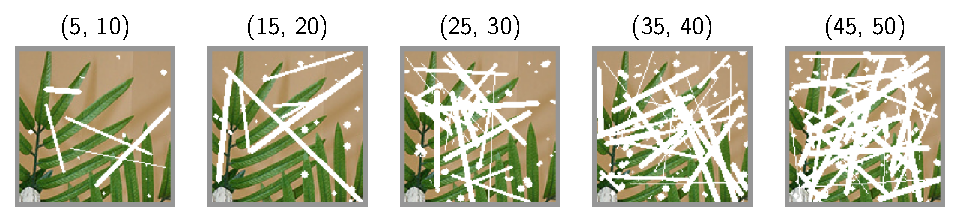
\includegraphics[width=\textwidth]{preliminary-work/masked1.pdf}
        \caption{Images affected by masks generated using random shapes}
        \label{fig:random_shapes_masked}
    \end{subfigure}
    \vskip\baselineskip
    \begin{subfigure}[ht]{\linewidth}
        \centering
        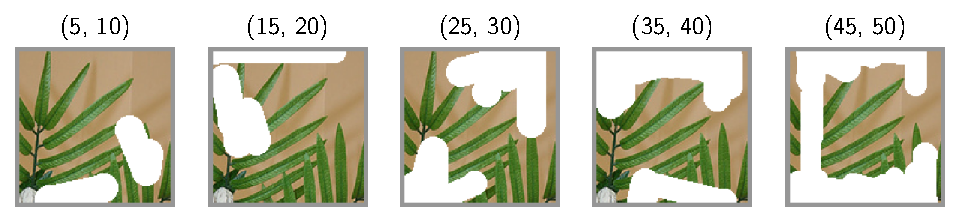
\includegraphics[width=\textwidth]{preliminary-work/masked2.pdf}
        \caption{Images affected by masks generated using the modified freeform algorithm}
        \label{fig:freeform_masked}
    \end{subfigure}
    \caption{Example of a cropped image masked with different degradation ratio intervals}
    \label{fig:masked-comp}
\end{figure}

\unnumberedsubsection{Normalization of images}

Following the masking process, the original image (referred to as the ground truth) and the masked image (the one designated for inpainting) are assembled into a \textbf{pair}. Following this pairing, each image undergoes an essential pre-processing step known as normalization, a fundamental procedure that involves scaling the initial values of the data to a specific range. This process is instrumental in reducing computational complexity and facilitating faster convergence of the learning algorithm.

In the absence of normalization, the range of pixel values could be considerably large (e.g. $[0, 255]$ for an 8-bit image), which could induce numerical instability during the learning process. By scaling the values to a smaller range, such issues can be effectively mitigated. Therefore, both the ground truth and the masked image in each pair are normalized in the $[0, 1]$ range, ensuring a stable and efficient learning process.


\unnumberedsubsection{Caching of the processed dataset}

The final stage in the pre-processing pipeline involves caching the processed image pairs. Caching is a technique that temporarily stores the processed data in a storage area, specifically the system's RAM in this case, to facilitate quicker access during subsequent processes. This step is particularly beneficial in enhancing the efficiency of the deep learning tasks by reducing the time taken to access the processed data. After the completion of the first epoch, the processed image pairs are cached into the system's RAM. This strategy ensures faster access times during the training process, thereby significantly improving the overall computational efficiency.

An additional reason for the implementation of caching in this context is the time-consuming nature of the mask generation process. Due to a limitation in the \texttt{TensorFlow} library, this process cannot be parallelized, resulting in an additional time overhead for mask generation. By caching the processed image pairs after the first epoch, the need to regenerate the masks for each epoch is eliminated, thereby saving considerable processing time. While the cache could also be stored on disk for larger size, the choice of RAM as the caching medium in this context offers the advantage of speed, which is crucial for the iterative nature of the training process and particularly beneficial given the time-intensive nature of the mask generation process.
